\begin{subsectionframemod}{Proposed Approaches}

    The main idea of DiffusionDet is to apply the diffusion principle to box generation.

    Random boxes are first sampled, and a model is trained to refine iteratively the size and position of the boxes so that they localize the objects in the input image.

    Specifically, the boxes are iteratively \alert{denoised} by the model.



    \begin{figure}
        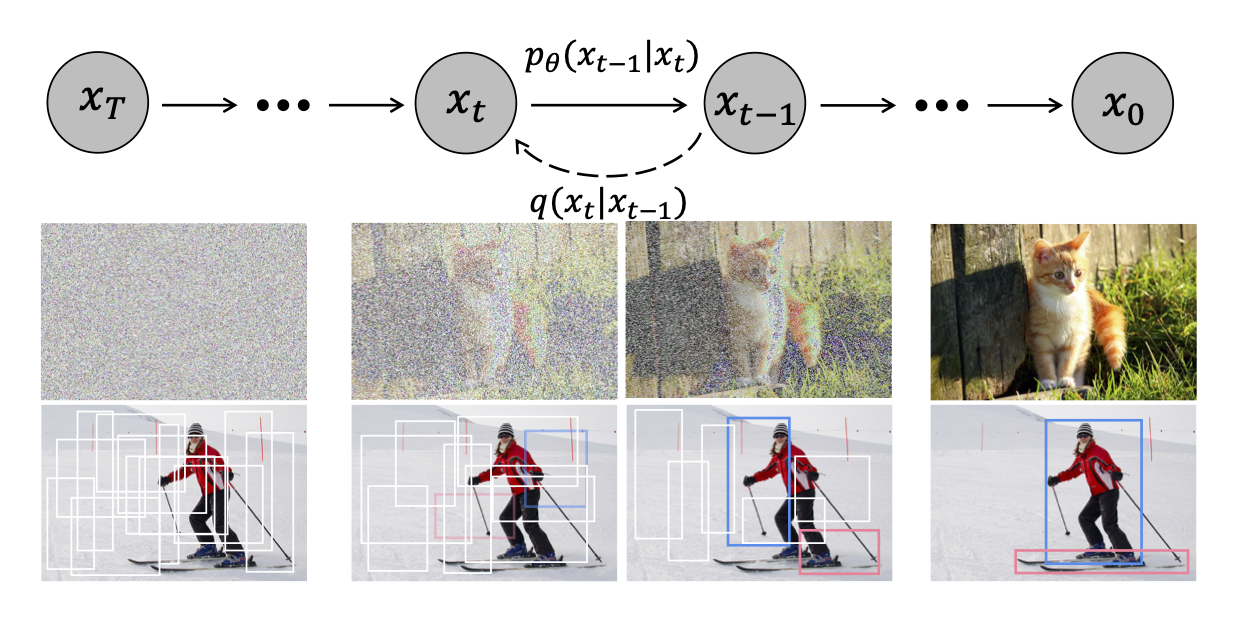
\includegraphics[width=0.70\textwidth]{Figures/teaser_diffusion}
        \caption{
        Diffusion model for object detection.
            In the first line a diffusion model where $q$ is the diffusion process and $p_{\theta}$ is the reverse process.
            Then a diffusion model for image generation task.
            And in the last one we propose to formulate object detection as a denoising diffusion process from noisy boxes to object boxes.\\
            \small{\textit{taken from DiffusionDet paper \cite{chen2022diffusiondet}}}
        }\label{fig:diffusion}
    \end{figure}

\end{subsectionframemod}

\begin{subsectionframemod}{Proposed Approaches}

    The denoising part of DiffusionDet is a lightweight hybrid network, it consists of a self-attention layer (transformer-like) followed by a dynamic layer (called an Instance Interaction layer).
    The detection head processes object features independently, but the Instance Interaction layer enables interactions between instances.
    The detection head is applied iteratively to refine the bounding boxes

    \begin{figure}
        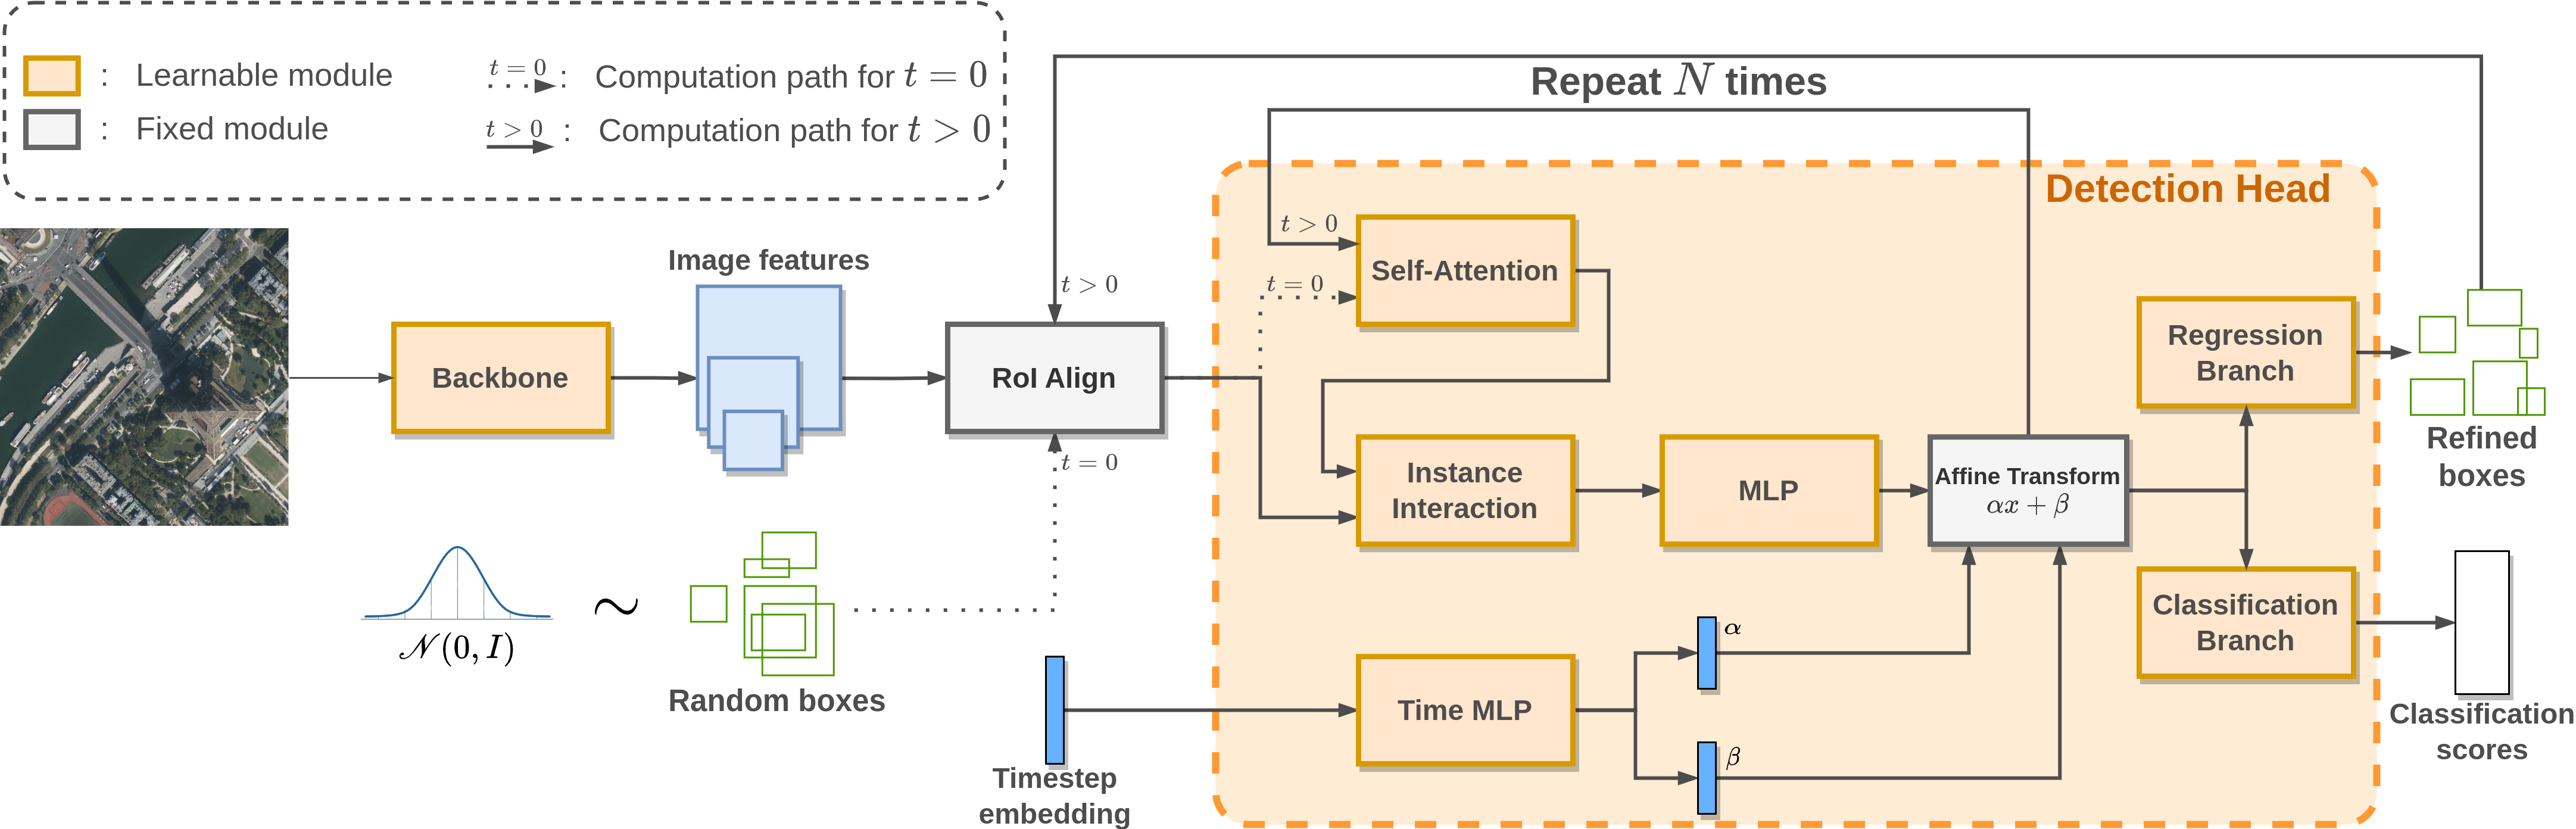
\includegraphics[width=0.95\textwidth]{Figures/DiffusionDet}
        \caption{DiffusionDet architecture and detailed detection head design.}\label{fig:diffusiondet}
    \end{figure}

\end{subsectionframemod}